\documentclass[a4paper]{article}

\usepackage{fullpage} % Package to use full page
\usepackage{parskip} % Package to tweak paragraph skipping
\usepackage{tikz} % Package for drawing
\usepackage{amsmath}
\usepackage{hyperref}
\usepackage{graphicx} % package for insert image

\title{Discover exons with highest SNP density}
\author{Edgar G. Nogales}
\date{10/28/2016}

\begin{document}

\maketitle
\section{Introduction}

In this case we will work with Galaxy tool. It's an open source, website platform where we can perform queries in a multiple bio-medical data-sets.

Differentiation is now a technique taught to mathematics students throughout the world. In this document I will discuss some aspects of differentiation.

\section{Exercise}

In this case we will work with 2 main databases. In the database "UCSC Main on Human: knownGene (genome)" we will find all the exons from the human genome. And in the data-set "UCSC Main on Human: snp147Common (genome)" will give us the SNPs of the human genome.\\

\centerline{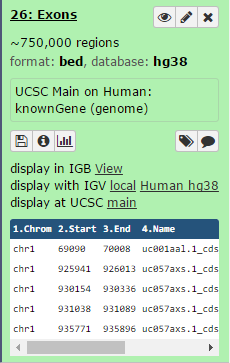
\includegraphics[scale=0.5]{26_Exons.png}
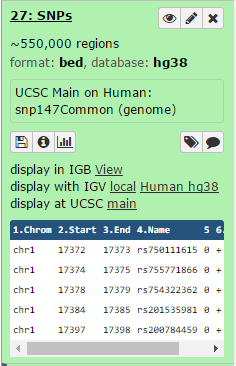
\includegraphics[scale=0.5]{27_SNPs.PNG}}

Once we have all the data we need, it's time to start working with it. Using the exon's table, we will calculate the size subtracting the position of the exons and adding 1.
To perform the operation we need to click on "Text Manipulation" >> "Compute an expression on every row" and we will fill the fields like in the image.\\

\centerline{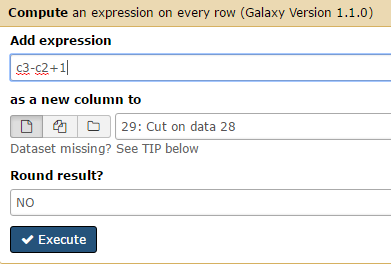
\includegraphics[scale=0.5]{28_compute.PNG}}

And the result will be like: \\

\centerline{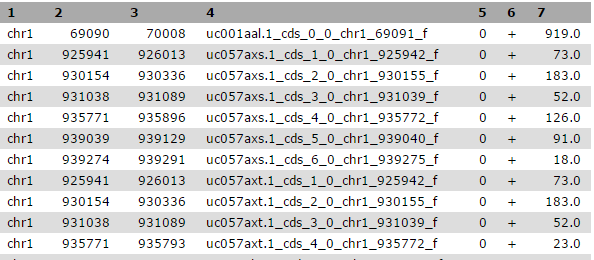
\includegraphics[scale=0.5]{28_table.PNG}}

Next step will be to count how many SNPs we find for each Exon. For that we will use the "Group by" command and then "count" the repetitions.\\

\centerline{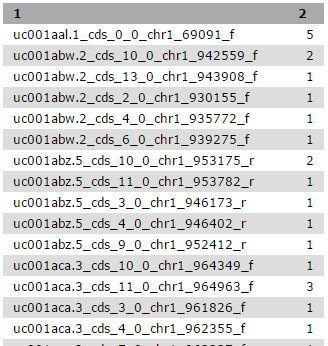
\includegraphics[scale=0.5]{33_SNP_Exon.PNG}}

Next step will be to join both tables. Here we find some problems because we used the command "Join two Datasets side by side on a specified field" and it generates too much data and Galaxy was not able to work with it. Finally we find that we need to use another command "Join the intervals of two datasets side-by-side"\\

\centerline{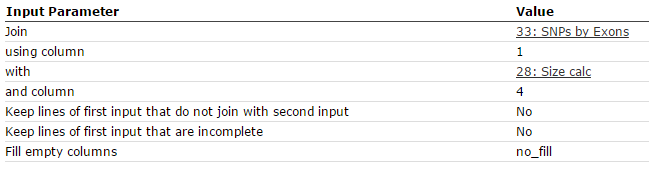
\includegraphics[scale=0.5]{34_join.PNG}}

To calculate the density of our data, we need to divide the number of SNPs by the size of the Exons\\

\centerline{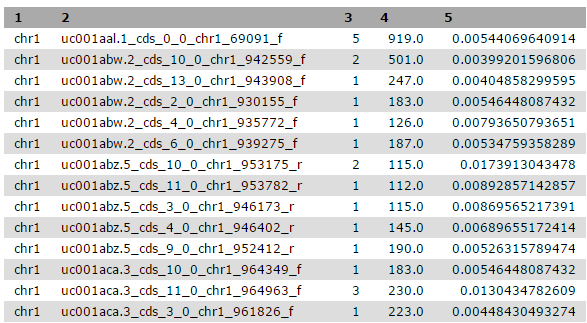
\includegraphics[scale=0.5]{37_density.PNG}}

Finally, we need to sort the result to have the highest density in the upper rows. For that we will use the "sort" function.\\

\centerline{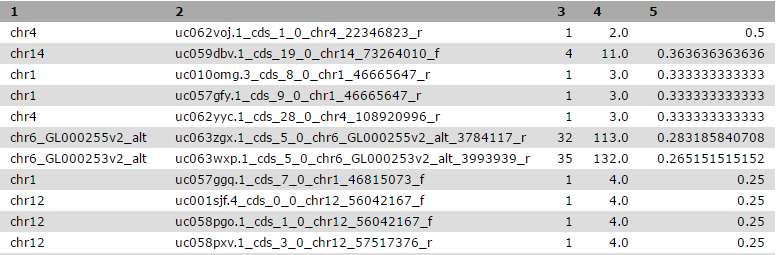
\includegraphics[scale=0.5]{result.PNG}}

We can see that the highest density is in chr4 Exon uc062voj because we can find 4 SNPs in just 2 bases.\\
After export the workflow, we have a flux like that\\

\centerline{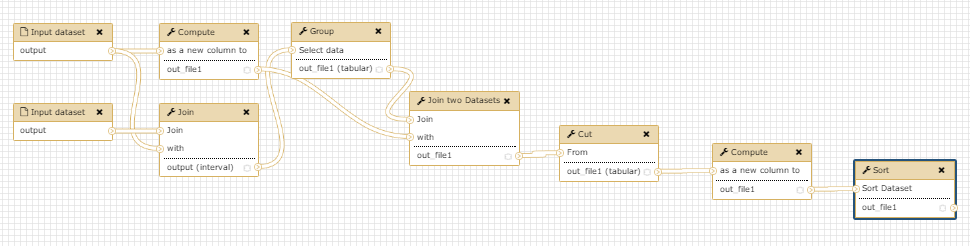
\includegraphics[scale=0.8]{workflow.PNG}}


\end{document}